% common part for every lection

\documentclass{beamer}

\usetheme{Warsaw}
\usefonttheme[onlylarge]{structurebold}
\setbeamerfont*{frametitle}{size=\normalsize,series=\bfseries}
\setbeamertemplate{navigation symbols}{}

\usepackage{pdfpages}
\usepackage{soul}
\usepackage{ucs}
\usepackage[utf8x]{inputenc}
\usepackage[TS1,T2A]{fontenc}
\usepackage[english,russian]{babel}
\usepackage{times}
\usepackage{listings}

\author[Author, Vlad Shakhov]{Влад 'mend0za' Шахов\\Linux \& Embedded Team Leader}

\institute[SaM Solutions]
{
  Linux \& Embedded Department
}

\date[Dec 2012]

\subject{Linux QA training}

\pgfdeclareimage[height=1.5cm]{sam-solutions-logo}{clipart/sam-solutions-elinux}

\logo{\pgfuseimage{sam-solutions-logo}}

\graphicspath{{./clipart/}}


\title[SaM Solutions. Linux QA Training]
{
  Занятие 1.\\
  Введение в Linux.
}

\begin{document}

\begin{frame}
  \titlepage
\end{frame}

% краткая историческая справка
\begin{frame}
  \frametitle{История Linux}

  \begin{enumerate}
    \item Начало. AT\&T Unix Version 2. 1971
    \item BSD (198x) (?)
    \item BSD 4.2. Первая реализация TCP/IP. 1982
    \item Расцвет коммерческих Unix-подобных систем.
    \item Проект GNU. 1985 
    \item Linux 1.0 1992 (?)
  \end{enumerate}

\end{frame}

% архитектура классических Unix
% картинки : круговая, и прямоугольная
\begin{frame}
  \frametitle{Архитектура классических Unix}
    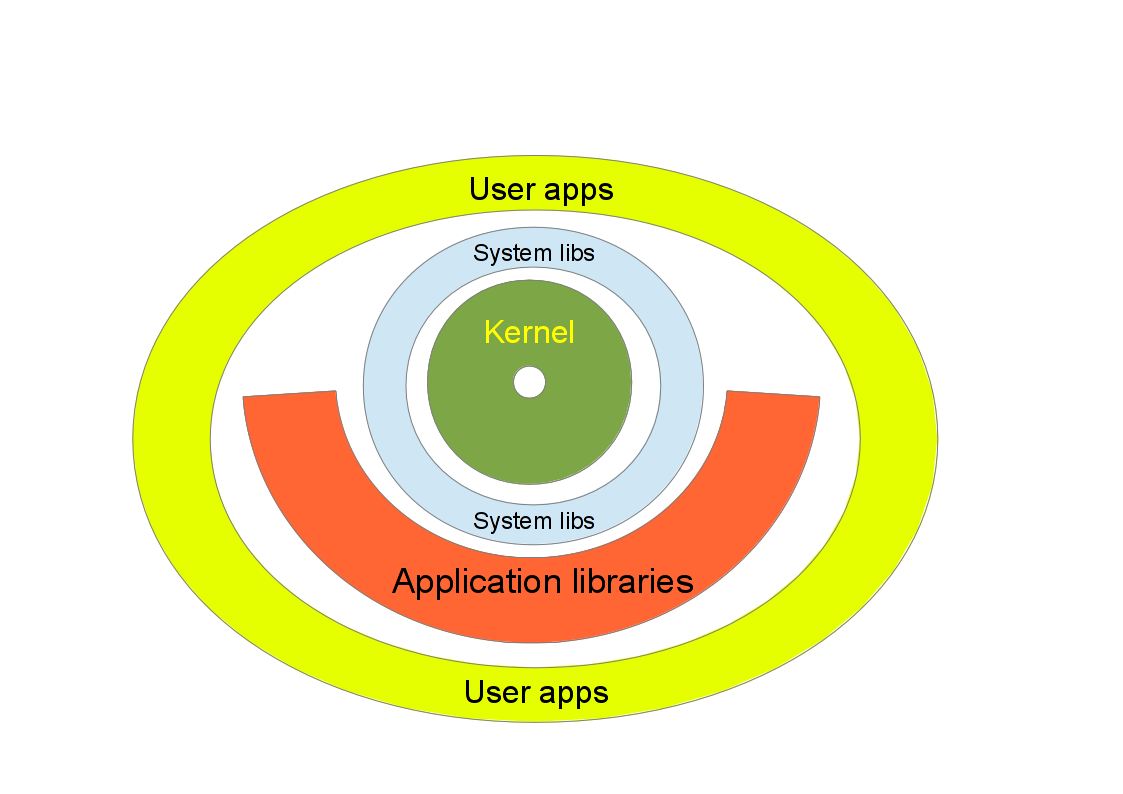
\includegraphics[height=8cm]{classic-unix-arch}
\end{frame}


\begin{frame}
  \frametitle{Архитектура Linux - 2}

  \begin{center}
    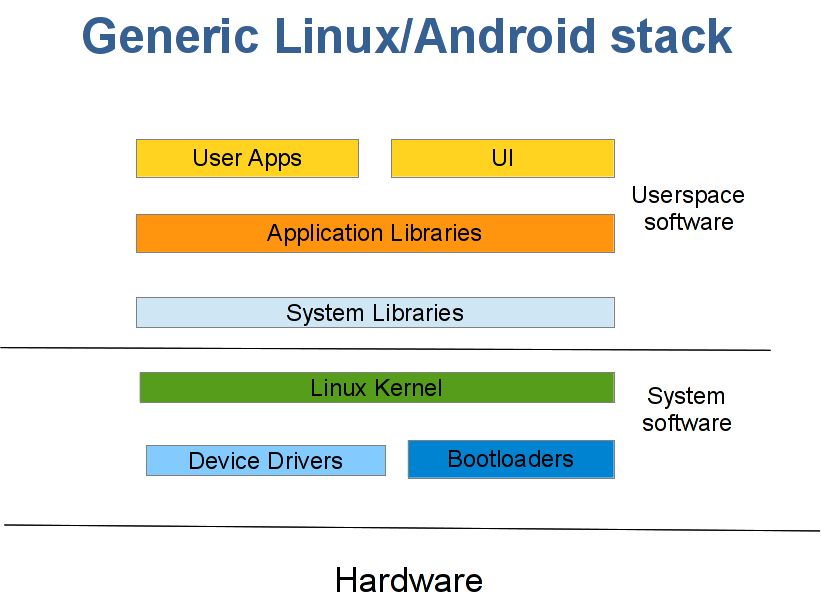
\includegraphics[height=7cm]{linux-software-stack}
  \end{center}
\end{frame}

% основные черты
\begin{frame}
  \frametitle{Основные черты Unix-подобных ОС}

  \begin{itemize}
    \item Многозадачная многопользовательская ОС.
    \item Переносимость: Код на языке Си
    \item Стандарты :
      \begin{itemize} 
	\item одинаковая структура ОС
	\item ряд стандартных, переносимых интерфейсов.
      \end{itemize}
    \item Командная строка - единый интерфейс управления.
    \item Eдиная древовидная файловая система\footnote{Через интерфейс файловой системы осуществляется доступ к данным, терминалам, принтерам, дискам, сети и даже к оперативной памяти}.
    \item Большое количество программного обеспечения.
  \end{itemize}
\end{frame}

% пользовательская сессия


\end{document}
